\section{EEG analysis \label{multimodal:data:eeg}}

First change directory to the EEG subdirectory (either in \matlab\, or via the ``CD'' option in the SPM ``Utils'' menu).

\subsection{Convert}

Press the \textsc{Convert} button and select the \texttt{faces\_run1.bdf} file. At the prompt ``Define settings?'' select ``just read''.
SPM will now read the original Biosemi format file and create an SPM compatible data file, called \texttt{spm8\_faces\_run1.mat} and \texttt{spm8\_faces\_run1.dat} in the current \matlab\ directory. After the conversion is complete the data file will be automatically opened in SPM8 reviewing tool. By default you will see the ``info'' tab. At the top of the window there is some basic information about the file. Below it you will see several clickable tabs with additional information. The ``history'' tab lists the processing steps that have been applied to the file. At this stage there is only one such step - conversion. The ``channels'' tab lists the channels in the file and their properties, the ``trial'' tab lists the trials or in the case of a continuous file all the triggers (events) that have been recorded. The ``inv'' tab is used for reviewing the inverse solutions and is not relevant for the time being. Note that the detailed information in the tabs will not be available for \matlab\ versions older than 7.4.  At the top of the window there is another set of tabs. If you click on the ``EEG'' tab you will see the raw EEG traces. They all look unusually flat because the continuous data we have just converted contains very low frequencies and baseline shifts. Therefore, if we try to view all the channels together, this can only be done with very low gain.
If you press the ``intensity rescaling'' button (with arrows pointing up and down) several times you will start seeing EEG activity in a few channels but the other channels will not be visible as they will go out of range. You can also use the controls at the bottom of the window to scroll through the recording. If you press the icon to the right of the mini-topography icon, with the rightwards pointing arrow, the display will move to the next trigger, shown as a vertical line through the display. (New triggers/events can be added by the rightmost icon). At the bottom of the display is a plot of the global field power across the session, with the black line indicating the current timewindow displayed (the width of this timewindow can be controlled by the two leftmost top icons).

\subsection{Downsample}

Here, we will downsample the data in time. This is useful when the data were acquired like ours with a high sampling rate of 2048 Hz. This is an unnecessarily high sampling rate for a simple evoked response analysis, and we will now decrease the sampling rate to 200 Hz, thereby reducing the file size by more than ten fold and greatly speeding up the subsequent processing steps. This step requires the Signal Processing toolbox. Select \textsc{Downsample} from the ``Other'' drop-down menu and select the \texttt{spm8\_faces\_run1.mat} file. Choose a new sampling rate of 200 (Hz). The progress bar will appear and the resulting data will be saved to files \texttt{dspm8\_faces\_run1.mat} and \texttt{dspm8\_faces\_run1.dat}. Note that this dataset and other intermediate datasets created during preprocessing will not be automatically opened in the reviewing tool, but you can always review them by selecting \texttt{M/EEG} from the ``Display'' drop down menu and choosing the corresponding \texttt{.mat} file.

\subsection{Montage}

In this step, we will identify the VEOG and HEOG channels, remove several channels that don't carry EEG data and are of no importance to the following and convert the 128 EEG channels to ``average reference'' by subtracting the mean of all the channels from each channel\footnote{Re-referencing EEG to the mean over EEG channels is important for source localisation. Note also that if some channels are subsequently marked ``bad'' (see later), one should re-reference again, because bad channels are ignored in any localisation.}. We generally recommend removal of data channels that are no longer needed because this will reduce the total file size and conversion to average reference is necessary at present for source modelling to work correctly. To do so, we use the \textsc{montage} tool in SPM, which is a general approach for pre-multiplying the data matrix (channels $\times$ time) by another matrix that linearly weights all channel data. This provides a very general method for data transformation in M/EEG analysis.

The appropriate montage-matrix can be specified in SPM by either using a graphical interface, or by supplying the matrix saved in a file. We will do the latter. The script to generate this file is \texttt{faces\_eeg\_montage.m}. Running this script will produce a file named \texttt{faces\_eeg\_montage.mat}. In our case, we would like to keep only channels 1 to 128. To re-reference each of these to their average, the script uses \matlab\ ``detrend'' to remove the mean of each column (of an identity matrix). In addition, there were four EOG channels (131, 132, 135, 136), where the HEOG is computed as the difference between channels 131 and 132, and the VEOG by the difference between channels 135 and 136. 

You now call the montage function by choosing \textsc{Montage} in the ``Other'' drop-down menu and:
\begin{itemize}
\item Select the M/EEG-file \texttt{dspm8\_faces\_run1.mat}.
\item ``How to specify the montage ?'' Answer ``file''.
\item Then select the generated \texttt{faces\_eeg\_montage.mat} file.
\item ``Keep the other channels?'' : ``No''.
\end{itemize}
This will remove the uninteresting channels from the data. The progress bar appears and SPM will generate two new files \texttt{Mdspm8\_faces\_run1.mat} and \texttt{Mdspm8\_faces\_run1.dat}.

\subsection{Epoch}
To epoch the data click on \textsc{Epoching}. Select the \texttt{Mdspm8\_faces\_run1.mat} file. Choose the peri-stimulus time window, first the start \texttt{-200}, then the end \texttt{600} ms. Choose 1 condition. There is no information in the file at this stage to distinguish between faces and scrambled faces. We will add this information at a later stage. You can give this condition any label, for instance ``stim''. A GUI pops up which gives you a complete list of all events in the EEG file. Each event has type and value which might mean different things for different EEG and MEG systems. So you should be familiar with your particular system to find the right trigger for epoching. In our case it is not very difficult as all the events but one appear only once in the recording, whereas the event with type ``STATUS'' and value 1 appears 172 times which is exactly the number of times a visual stimulus was presented. Select this event and press OK. Answer two times ``no'' to the questions ``review individual trials'', and ``save trial definitions''. The progress bar will appear and the epoched data will be saved to files \texttt{eMdspm8\_faces\_run1.mat} and \texttt{eMdspm8\_faces\_run1.dat}. The epoching function also performs baseline correction by default (with baseline -200 to 0ms). Therefore, in the epoched data the large channel-specific baseline shifts are removed and it is finally possible to see the EEG data clearly in the reviewing tool.

\subsection{Reassignment of trial labels}

Open the file \texttt{eMdspm8\_faces\_run1.mat} in the reviewing tool (under ``Display'' button). The first thing you will see is that in the history tab there are now 4 processing steps. Now switch to the ``trials'' tab. You will see a table with 172 rows - exactly the number of events we selected before. In the first column the label ``stim'' appears in every row. What we would like to do now is change this label to ``faces'' or ``scrambled'' where appropriate. We should first open the file \texttt{condition\_labels.txt} (in the EEG directory) with any text editor, such as \matlab\ editor or Windows notepad. In this file there are exactly 172 rows with either ``faces'' or ``scrambled'' in each row. Select and copy all the rows (Ctrl-A, Ctrl-C on Windows). Then go back to SPM and the trials tab. Place the cursor in the first row and first column cell with the ``stim'' label and paste the copied labels (Ctrl-V). The new labels should now appear for all rows. Press the ``update'' button above the table and then the ``SAVE'' button at the top right corner of the window. The new labels are now saved in the dataset.

\subsection{Using the history and object methods to preprocess the second file}

At this stage we need to repeat the preprocessing steps for the second file \texttt{faces\_run2.bdf}. You can do it by going back to the ``Convert'' section and repeating all the steps for this file, but there is a more efficient way. If you have been following the instructions until now the file \texttt{eMdspm8\_faces\_run1.mat} should be open in the reviewing tool. If it is not the case, open it. Go to the ``history'' tab and press the ``Save as script'' button. A dialog will appear asking for the name of the \matlab\ script to save. Let's call it \texttt{eeg\_preprocess.m}. Then there will be another dialogue suggesting to select the steps to save in the script. Just press ``OK'' to save all the steps. Now open the script in the \matlab\ editor. You will now need to make some changes to make it work for the second file. Here we suggest the simplest way to do it that does not require familiarity with \matlab\ programming. But if you are more familar with \matlab\ you'll definitely be able to do a much better job. First, replace all the occurences of ``run1'' in the file with ``run2''. You can use the ``Find \& Replace'' functionalty (Ctrl-F) to do it. Secondly, erase the line starting with \texttt{S.timewindow} (line 5). This line defines the time window to read, in this case from the first to the last sample of the first file. The second file is slightly longer than the first so we should let SPM determine the right time window automatically. Save the changes and run the script by pressing the ``Run'' button or writing \texttt{eeg\_preprocess} in the command line. SPM will now automatically perform all the steps we have done before using the GUI. This is a very easy way for you to start processing your data automatically once you come up with the right sequence of steps for one file. After the script finishes running there will be a new set of files in the current directory including \texttt{eMdspm8\_faces\_run2.mat} and \texttt{eMdspm8\_faces\_run2.dat}. If you open these files in the reviewing tool and go to the ``trials'' tab you will see that the trial labels are still ``stim''. The reason for this is that updates done using the reviewing tool are not presently recorded in the history (with the exception of the ``Prepare'' interface, see below). You can still do this update automatically and add it to your script. If you write \texttt{D} in the command line just after running the script and press ``Enter'' you will see some information about the dataset \texttt{eMdspm8\_faces\_run2}. \texttt{D} is an object, this is a special kind of data structure that makes it possible to keep different kinds of related information (in our case all the properties of our dataset) and define generic ways of manipulating these properties. For instance we can use the command:
\begin{verbatim}
D = conditions(D, [], importdata('condition_labels.txt')); D.save;
\end{verbatim}
to update the trial labels using information imported from the \texttt{condition\_labels.txt}\footnote{You might need to change the full path to this text file inside the single quotes, depending on your current directory and the directory of the original data.} (the two runs had identical trials). Now, \texttt{conditions}' is a ``method'', a special function that knows where to store the labels in the object. All the methods take the M/EEG object (usually called \texttt{D} in SPM by convention) as the first argument. The second argument is a list of indices of trials for which we want to change the label. We specify an empty matrix which is interpreted as ``all''. The third argument is the new labels which are imported from the text file using a \matlab\ built-in function. We then save the updated dataset on disk using the \texttt{save} method. If you now write \texttt{D.conditions} or \texttt{conditions(D)} (which are two equivalent ways of calling the \texttt{conditions} method with just D as an argument), you should see a list of 172 labels, either ``faces'' or ``scrambled''. If you add the commands above at the end of your automatically generated script, you can run it again and this time the output will have the right labels.

\subsection{Merge}

We will now merge the two epoched files we have generated until now and continue working on the merged file. Select the ``Merge'' command from the ``Other'' drop-down menu. In the selection window that comes up click on \texttt{eMdspm8\_faces\_run1.mat} and \texttt{eMdspm8\_faces\_run2.mat}. Press ``done''. Answer ``Leave as they are'' to ``What to do with condition labels?''. This means that the trial labels we have just specified will be copied as they are to the merged file. A new dataset will be generated called \texttt{ceMdspm8\_faces\_run1.\{mat,dat\}}.

\subsection{Prepare}

In this section we will add the separately measured electrode locations and headshape points to our merged dataset. In principle, this step is not essential for further analysis because SPM8 automatically assigns electrode locations for commonly used EEG caps and the Biosemi 128 cap is one of these. Thus, default electrode locations are present in the dataset already after conversion. But since these locations are based on channel labels they may not be precise enough and in some cases may be completely wrong because sometimes electrodes are not placed in the correct locations for the corresponding channel labels. This can be corrected by importing individually measured electrode locations. Select \textsc{Prepare} from the ``Other'' menu and in the file selection window select \texttt{ceMdspm8\_faces\_run1.mat}. A menu will appear at the top of SPM interactive window (bottom left window). In the ``Sensors'' submenu choose ``Load EEG sensors''/``Convert locations file''. In the file selection window choose the \texttt{electrode\_locations\_and\_headshape.sfp} file (in the original EEG directory). Then from the ``2D projection'' submenu select ``Project 3D (EEG)''. A 2D channel layout will appear in the Graphics window. Select ``Apply'' from ``2D Projection'' and ``Save'' from ``File'' submenu. Note that the same functionality can also be accessed from the reviewing tool by pressing the ``Prepare SPM file'' button.

\subsection{Artefact rejection}

Here we will use SPM8 artefact detection functionality to exclude from analysis trials contaminated with large artefacts. Press the \textsc{Artefacts} button. A window of the SPM8 batch interface will open. You might already be familiar with this interface from other SPM8 functions. It is also possible to use the batch interface to run the preprocessing steps that we have performed until now, but for artefact detection this is the only graphical interface and there is no way to configure it with the usual GUI buttons. Click on ``File name'' and select the \texttt{ceMdspm8\_faces\_run1.mat} file.  Double click ``How to look for artefacts'' and a new branch will appear. It is possible to define several sets of channels to scan and several different methods for artefact detection. We will use simple thresholding applied to all channels. Click on ``Detection algorithm'' and select ``Threshold channels'' in the small window below. Double click on ``Threshold'' and enter 200 (in this case $\mu V$). The batch is now fully configured. Run it by pressing the green button at the top of the batch window.

This will detect trials in which the signal recorded at any of the channels exceeds 200 microvolts (relative to pre-stimulus baseline). These trials will be marked as artefacts. Most of these artefacts occur on the VEOG channel, and reflect blinks during the critical time window. The procedure will also detect channels in which there is a large number of artefacts (which may reflect problems specific to those electrodes, allowing them to be removed from subsequent analyses).

In this case, the \matlab\ window will show:
\begin{verbatim}
    There isn't a bad channel.
    39 rejected trials: 38   76   82   83   86   88   89   90   92   [...]
\end{verbatim}
(leaving 305 valid trials). A new file will also be created, \texttt{aceMdspm8\_faces\_run1.\{mat,dat\}}.

\subsection{Exploring the M/EEG object}

We can now review the preprocessed dataset from the \matlab\ command line by typing:
\begin{verbatim}
    D = spm_eeg_load
\end{verbatim}
and selecting the \texttt{aceMdspm8\_faces\_run1.mat} file. This will print out some basic information about the M/EEG object \texttt{D} that has been loaded into \matlab\ workspace.
\begin{verbatim}
    SPM M/EEG data object
    Type: single
    Transform: time
    2 conditions
    130 channels
    161 samples/trial
    344 trials
    Sampling frequency: 200 Hz
    Loaded from file  ...\EEG\aceMdspm8_faces_run1.mat
    Use the syntax D(channels, samples, trials) to access the data.
\end{verbatim}

Note that the data values themselves are memory-mapped from \verb!aceMdspm8_faces_run1.dat! and can be accessed by indexing the \texttt{D} object (e.g, \texttt{D(1,2,3)} returns the field strength in the first sensor at the second sample point during the third trial). You will see that there are 344 trials (\texttt{D.ntrials}). Typing \texttt{D.conditions} will show the list of condition labels consisting of 172 faces (``faces'') and 172 scrambled faces (``scrambled''). \texttt{D.reject} will return a $1\times 344$ vector of ones (for rejected trials) and zeros (for retained trials). \texttt{D.condlist} will display a list of unique condition labels. The order of this list is important because every time SPM needs to process the conditions in some order, this will be the order. If you type \texttt{D.chanlabels}, you will see the order and the names of the channels. \texttt{D.chantype} will display the type for each channel (in this case either ``EEG'' or ``EOG''). \texttt{D.size} will show the size of the data matrix, [130 161 344] (for channels, samples and trials respectively). The size of each dimension separately can be accessed by \texttt{D.nchannels}, \texttt{D.nsamples} and \texttt{D.ntrials}. Note that although the syntax of these commands is similar to those used for accessing the fields of a struct data type in \matlab\, what's actually happening here is that these commands evoke special functions called ``methods'' and these methods  collect and return the requested information from the internal data structure of the \texttt{D} object. The internal structure is not accessible directly when working with the object. This mechanism greatly enhances the robustness of SPM code. For instance you don't need to check whether some field is present in the internal structure. The methods will always do it automatically or return some default result if the information is missing without causing an error.

Type \texttt{methods('meeg')} for the full list of methods performing operations with the object. Type \texttt{help meeg/method\_name} to get help about a method.


\subsection{Basic ERPs}

Press the \textsc{Averaging} button and select the \texttt{aceMdspm8\_faces\_run1.mat} file. At this point you can perform either ordinary averaging or ``robust averaging'' (Wager et al., 2005). Robust averaging makes it possible to suppress artefacts automatically without rejecting trials or channels completely, but just the contaminated parts. Thus, in principle we could do robust averaging without rejecting trials with eye blinks and this is something you can do as an exercise and see how much difference the artefact rejection makes with ordinary averaging vs. robust averaging. For robust averaging answer ``yes'' to ``Use robust averaging?''. Answer ``yes'' to ``Save weights'', and ``no'' to ``Compute weights by condition''\footnote{When there are approximately equal numbers of trials in each condition, as here, it is probably safer to compute weights across all conditions, so as not to introduce artifactual differences between conditions. However, if one condition has fewer trials than the others, it is likely to be safer to estimate the weights separately for each condition, otherwise evoked responses in the rarer condition will be downweighted so as to become more similar to the more common condition(s).}.

Finally, press ``Enter'' to accept the default ``Offset of the weighting function''. A new dataset will be generated \texttt{maceMdspm8\_faces\_run1.\{mat,dat\}} (``m'' for ``mean'') and automatically opened in the reviewing tool so that you can examine the ERP. There will also be an additional dataset named \texttt{WaceMdspm8\_faces\_run1.\{mat,dat\}}. This dataset will contain the weights used by robust averaging. This is useful to see what was suppressed and whether there might be some condition-specific bias that could affect the results.

Select ``Contrast'' from the ``Other'' pulldown menu on the SPM window. This function creates linear contrasts of ERPs/ERFs. Select the \texttt{maceMdspm8\_\-faces\_\-run1.mat} file,  enter $[1\: -1]$ as the first contrast and label it ``Difference'', answer ``yes'' to ``Add another'',  enter $[1/2\: 1/2]$ as the second contrast and label it ``Mean''. Press ``no'' to the question ``Add another'' and not to ``weight by num replications''. This will create new file \texttt{wmaceMdspm8\_faces\_run1.\{mat,dat\}}, in which the first trial-type is now the differential ERP between faces and scrambled faces, and the second trial-type is the average ERP for faces and scrambled faces.

To look at the differential ERP, again press ``Display: M/EEG'', and select the \texttt{wmaceMdspm8\_\-faces\_\-run1.mat} file. Switch to the ``EEG'' tab and to ``scalp'' display by toggling a radio button at the top of the tab. The Graphics window should then show the ERP for each channel (for Trial 1 the ``Difference'' condition). Hold SHIFT and select Trial 2 to see both conditions superimposed. Then click on the zoom button and then on one of the channels (e.g, ``B9'' on the bottom right of the display) to get a new window with the data for that channel expanded, as in Figure~\ref{multimodal:fig:4}.

\begin{figure}
\begin{center}
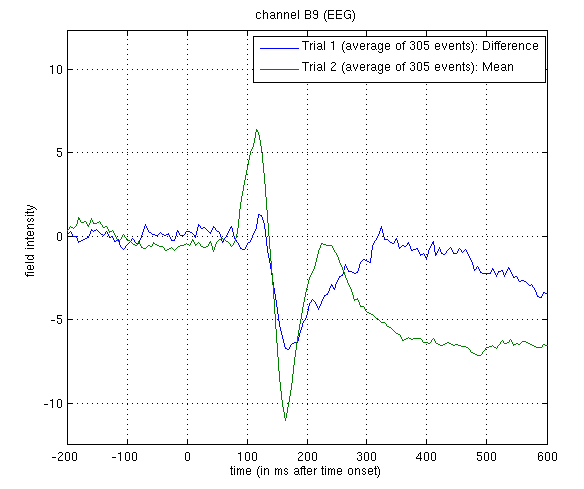
\includegraphics[width=100mm]{multimodal/figures/eeg_erp}
\caption{\em  Average (green) and differential (blue) ERPs for faces and scrambled faces at channel B9 in \texttt{wmaceMdspm8\_faces\_run1.mat}. \label{multimodal:fig:4}}
\end{center}
\end{figure}

The green line shows the average ERP evoked by faces and scrambled faces (at this occipitotemporal channel). A P1 and N1 are clearly seen. The blue line shows the differential ERP between faces and scrambled faces. The difference is small around the P1 latency, but large and negative around the N1 latency. The latter likely corresponds to the ``N170'' (Henson et al, 2003). We will try to localise the cortical sources of the P1 and N170 in Section~\ref{multimodal:eeg:3D}.

To see the topography of the differential ERP, click on Trial 1 again, press the ``topography'' icon button at the top of the window and scroll the latency from baseline to the end of the epoch. You should see a maximal difference around 180ms as in Figure~\ref{multimodal:fig:5} (possibly including a small delay of about 8ms for the CRT display to scan to the centre of the screen).

\begin{figure}
\begin{center}
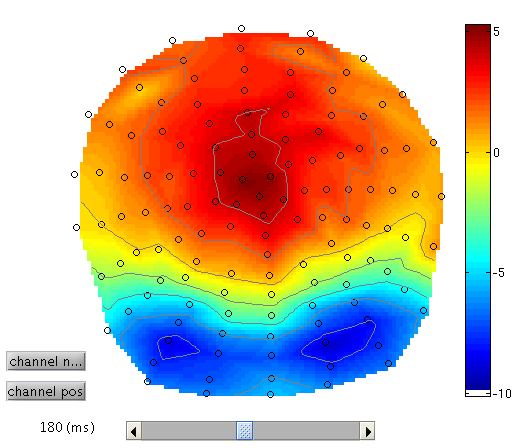
\includegraphics[width=100mm]{multimodal/figures/eeg_topo}
\caption{\em 2D topography for faces minus scrambled faces at 180ms. \label{multimodal:fig:5}}
\end{center}
\end{figure}

\subsection{3D SPMs (Sensor Maps over Time) \label{multimodal:eeg:3DSPM}}

A feature of SPM is the ability to use Random Field Theory to correct for multiple statistical comparisons across N-dimensional spaces. For example, a 2D space representing the scalp data can be constructed by flattening the sensor locations (using the 2D layout we created earlier) and interpolating between them to create an image of $M\times M$ pixels (when $M$ is user-specified, eg $M=32$). This would allow one to identify locations where, for example, the ERP amplitude in two conditions at a given timepoint differed reliably across subjects, having corrected for the multiple t-tests performed across pixels. That correction uses Random Field Theory, which takes into account the spatial correlation across pixels (i.e, that the tests are not independent). This kind of analysis is described earlier in the SPM manual, where a 1st-level design is used to create the images for a given weighting across timepoints of an ERP/ERF, and a 2nd-level design can then be used to test these images across subjects.

Here, we will consider a 3D example, where the third dimension is time, and test across trials within the single subject. We first create a 3D image for each trial of the two types, with dimensions $M\times M\times S$, where S=161 is the number of samples. We then take these images into an unpaired t-test across trials (in a 2nd-level model) to compare faces versus scrambled faces. We can then use classical SPM to identify locations in space and time in which a reliable difference occurs, correcting across the multiple comparisons entailed. This would be appropriate if, for example, we had no a priori knowledge where or when the difference between faces and scrambled faces would emerge\footnote{Note that the 2D location in sensor space for EEG will depend on the choice of montage.}.

Select the ``Convert to images'' option in the ``Other'' menu in the SPM main window, and select the \texttt{aceMdspm8\_faces\_run1.mat} file. You will then be prompted for ``output image dimensions'', for which you can accept the default of 32 (leading to a $32\times 32$ pixel space). It will then ask whether you want to interpolate or mask out bad channels, for which you select ``interpolate'' (though it will make no difference here because there are no bad channels).

This will take some time as it writes out an image for each trial (except rejected trials), in a new directory called \texttt{aceMdspm8\_faces\_run1}, which will itself contain two subdirectories, one for each trialtype. In each trialtype subdirectory there will be image and header files for each non-rejected trial of that type, e.g, \texttt{trial0002.\{hdr,img\}}. You can press ``Display: images'' to view one of these images - it will have dimensions $32\times 32\times 161$, with the origin set at [16 18.6 41] (where 41 samples is 0ms), as in Figure~\ref{multimodal:fig:6}.

\begin{figure}
\begin{center}
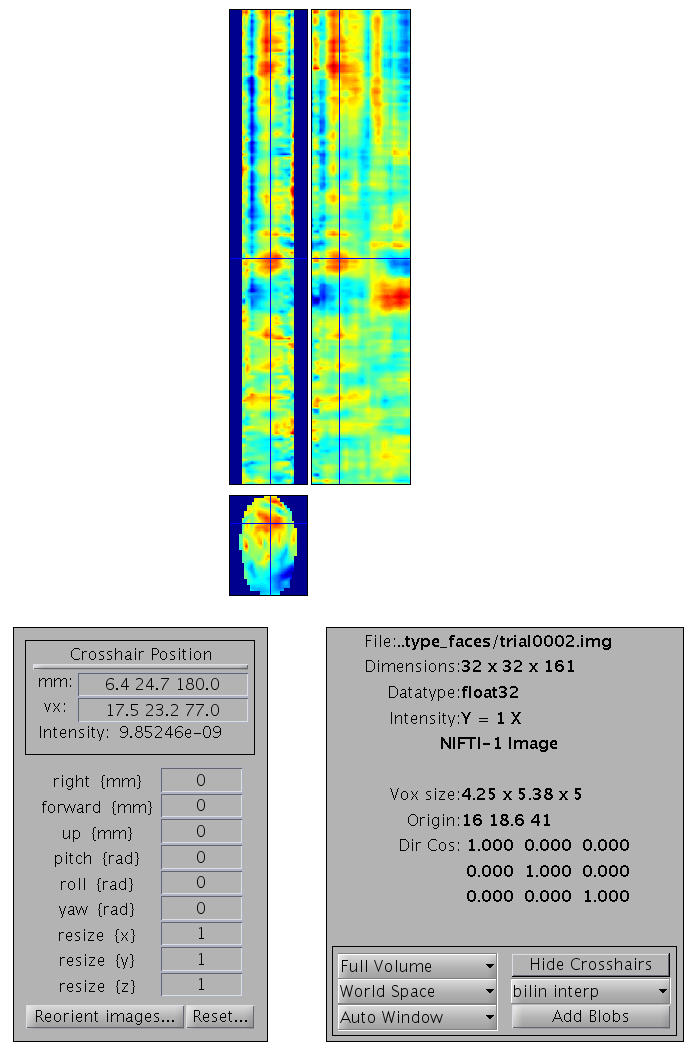
\includegraphics[width=120mm]{multimodal/figures/eeg_scalptime}
\caption{\em 3D image for trial 2 of \texttt{aceMdspm8\_faces\_run1.mat}. The bottom image is a 2D x-y space interpolated from the flattened electrode locations (at one point in time). The two top images are sections through x and y respectively, now expressed over time (vertical (z) dimension).\label{multimodal:fig:6}}
\end{center}
\end{figure}


\subsubsection{Smoothing \label{multimodal:eeg:3Dsmooth}}

Note that you can also smooth these images in 3D (i.e, in space and time) by pressing ``Smooth Images'' from the ``Others'' pulldown menu. When you get the Batch Editor window, you can enter a smoothness of your choice (eg [9 9 20], or 9mm by 9mm by 20ms). Note that you should also change the default ``Implicit masking'' from ``No'' to ``Yes''; this is to ensure that the smoothing does not extend beyond the edges of the topography.

As with fMRI, smoothing can improve statistics if the underlying signal has a smoothness close to the smoothing kernel (and the noise does not; the matched filter theorem). Smoothing may also be necessary if the final estimated smoothness of the SPMs (below) is not at least three times the voxel size; an assumption of Random Field Theory. In the present case, the data are already smooth enough (as you can check below), so we do not have to smooth further.


\subsubsection{Stats \label{multimodal:eeg:3Dstats}}

To perform statistics on these images, first create a new directory, eg. \texttt{mkdir XYTstats}.

Then press the ``Specify 2nd level'' button, to produce the batch editor window again. Select the new \texttt{XYTstats} as the ``Directory'', and ``two-sample t-test'' (unpaired t-test) as the ``Design''. Then select the images for ``group 1 scans'' as all those in the subdirectory ``type\_faces'' (using right click, and ``select all'') and the images for ``group 2 scans'' as all those in the subdirectory ``type\_scrambled''. You might want to save this batch specification, but then press ``run''\footnote{Note that we can use the default ``nonsphericity'' selections, i.e, that the two trial-types may have different variances, but are uncorrelated.}.

This will produce the design matrix for a two-sample t-test.

Then press ``Estimate'', and when it has finished, press ``Results'' and define a new F-contrast as [1 -1]. Keep the default contrast options, but threshold at $p<.05$ FWE corrected for the whole search volume and select ``Scalp-Time'' for the ``Data Type''. Then press ``whole brain'', and the Graphics window should now look like that in Figure~\ref{multimodal:fig:7}.

This will reveal ``regions'' within the 2D sensor space and within the -200ms to 600ms epoch in which faces and scrambled faces differ reliably, having corrected for multiple F-tests across pixels and time. There are a number of such regions, but the largest has maxima at [-13 -78 180] and [21 -68 180], corresponding to left and right posterior sites at 180ms. 

To relate these coordinates back to the original sensors, right-click in some white space in the top half of the Graphics window, to get a menu with various options. First select ``goto global maxima''. The red cursor should move to coordinates [-13, -78, 180]. (Note that you can also overlap the sensor names on the MIP by selecting ``display/hide channels'' - though it can get a bit crowded!). Then right-click again to get the same menu, but this time select ``go to nearest suprathreshold channel''. You will be asked to select the original EEG/MEG file used to create the SPM, which in this case is the \texttt{aceMdspm8\_faces\_run1.mat} file. This should output in the Matlab window:

\begin{verbatim}
	spm_mip_ui:	Jumped 4.25mm from [-13, -78, 180],
			to nearest suprathreshold channel (A15) at [ -8, -78, 180]
\end{verbatim}
In other words, it is EEG channel ``A15'' that shows the greatest face/scrambled difference over the epoch (itself maximal at 180ms).

Note that an F-test was used because the sign of the difference reflects the polarity of the ERP difference, which is not of primary interest (and depends on the choice of reference). Indeed, if you plot the contrast of interest from the cluster maxima, you will see that the difference is negative for the first posterior, cluster but positive for the second, central cluster. This is consistent with the polarity of the differences in Figure~\ref{multimodal:fig:5}\footnote{The former likely corresponds to the ``N170'', while the latter likely corresponds to the ``VPP'', which may be two signs of the same effect, though of course these effects depend on the choice of reference.}.

If one had more constrained a priori knowledge about where and when the N170 would appear, one could perform an SVC based on, for example, a box around posterior channels and between 150 and 200ms poststimulus. See \url{http://imaging.mrc-cbu.cam.ac.uk/meg/SensorSpm} for more details.

If you go to the global maximum, then press ``overlays'', ``sections'' and select the ``mask.img'' in the stats directory, you will get sections through the space-time image. A right click will reveal the current scalp location and time point. By moving the cursor around, you can see that the N170/VPP effects start to be significant (after whole-image correction) around 150ms (and may also notice a smaller but earlier effect around 100ms).

\begin{figure}
\begin{center}
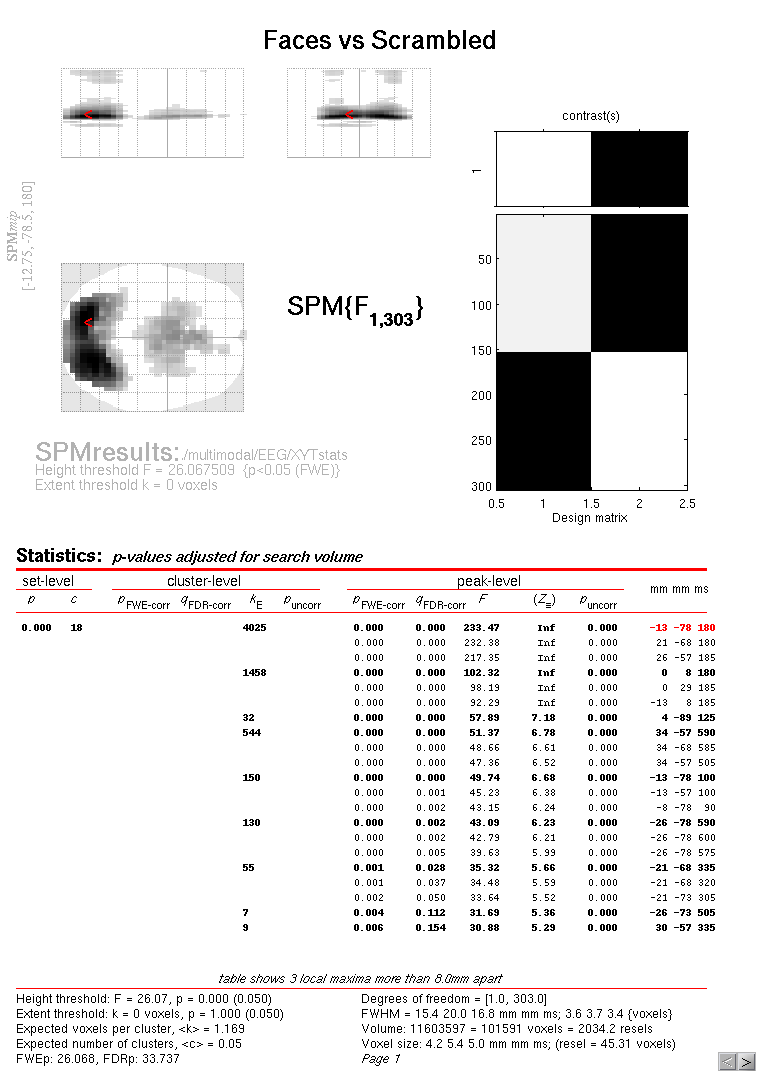
\includegraphics[width=120mm]{multimodal/figures/eeg_scalptime_results}
\caption{\em 3D sensor-time SPM{F} at $p<.05$ FWE corrected for the amplitude difference between face and scrambled face trials. The x, y coordinates refer to position in the 32x32 electrode plane (with units of mm); the z coordinate refers to peristimulus time in ms (to the nearest sampling of 5ms). \label{multimodal:fig:7}}
\end{center}
\end{figure}

\subsection{3D ``imaging'' reconstruction \label{multimodal:eeg:3D}}

Here we will demonstrate a distributed source reconstruction of the N170 differential evoked response between faces and scrambled faces, using a grey-matter mesh extracted from the subject's MRI, and the Multiple Sparse Priors (MSP) method in which multiple constraints on the solution can be imposed (Friston et al, 2008, Henson et al, 2009a).

Press the ``3D source reconstruction'' button, and press the ``load'' button at the top of the new window. Select the \verb!wmaceMdspm8_faces_run1.mat! file and type a label (eg "N170 MSP") for this analysis\footnote{Note that no new M/EEG files are created during the 3D reconstruction; rather, each step involves updating of the cell-array field \texttt{D.inv}, which will have one entry per analysis performed on that dataset (e.g, \texttt{D.inv\{1\}} in this case).}.

Press the ``MRI'' button, select the \texttt{smri.img} file within the \texttt{sMRI} sub-directory, and select ``normal'' for the cortical mesh.

The ``imaging'' option corresponds to a distributed source localisation, where current sources are estimated at a large number of fixed points (8196 for a ``normal'' mesh here) within a cortical mesh, rather than approximated by a small number of equivalent dipoles (the ECD option). The imaging  approach is better suited for group analyses and (probably) for later-occuring ERP components. The ECD approach may be better suited for very early sensory components (when only small parts of the brain are active), or for DCMs using a small number of regions (Kiebel et al, 2006).

The first time you use a particular structural image for 3D source reconstruction, it will take some time while the MRI is segmented (and normalisation parameters determined). This will create in the \texttt{sMRI} directory the files \texttt{y\_smri.nii} and \texttt{smri\_seg8.mat} for normalisation parameters and 4 GIfTI (\texttt{.gii}) files defining the cortical mesh, inner skull, outer skull and scalp surface.

When meshing has finished, the cortex (blue), inner skull (red), outer skull (orange) and scalp (pink) meshes will be shown in the Graphics window with slices from the sMRI image, as shown in Figure~\ref{multimodal:fig:3}. This makes it possible to visually verify that the meshes fit the original image well. The field \texttt{D.inv\{1\}}.mesh field will be updated in \matlab\ . Press ``save'' in top right of window to update the corresponding \texttt{mat} file on disk.

\begin{figure}
\begin{center}
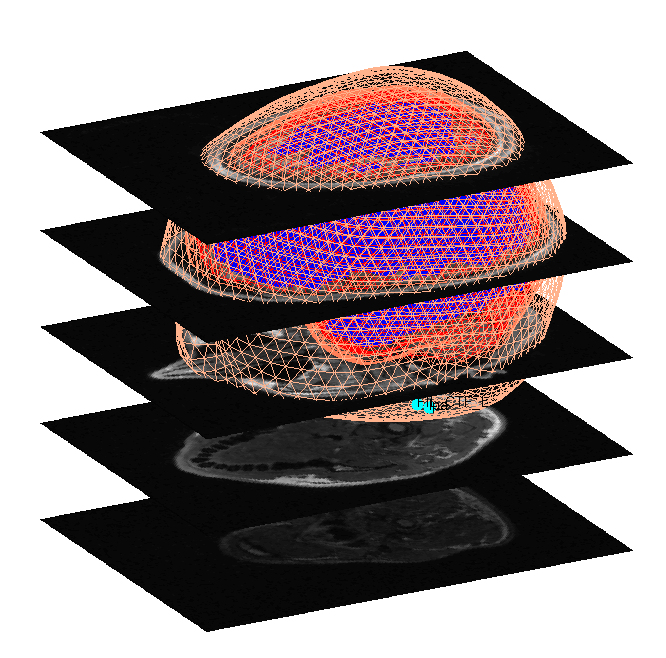
\includegraphics[width=90mm]{multimodal/figures/eeg_meshing}
\caption{\em Cortex (blue), inner skull (red), outer skull (orange) and scalp (pink) meshes with transverse slices of the subject's MRI. \label{multimodal:fig:3}}
\end{center}
\end{figure}

Both the cortical mesh and the skull and scalp meshes are not created directly from the segmented MRI, but rather are determined from template meshes in MNI space via inverse spatial normalisation (Mattout et al, 2007).

Press the ``Co-register'' button. You will first be asked to select at least 3 fiducials from a list of points in the EEG dataset (from Polhemus file): by default, SPM has already highlighted what it thinks are the fiducials, i.e, points labelled ``nas'' (nasion), ``lpa'' (left preauricular) and ``rpa'' (right preauricular). So just press ``ok''.

You will then be asked for each of the 3 fiducial points to specify its location on the MRI images. This can be done by selecting a corresponding point from a hard-coded list (``select''). These points are inverse transformed for each individual image using the same deformation field that is used to create the meshes. The other two options are typing the MNI coordinates for each point (``type'') or clicking on the corresponding point in the image (``click''). Here, we will type coordinates based on where the experimenter defined the fiducials on the \texttt{smri.img}. These coordinates can be found in the \texttt{smri\_fid.txt} file also provided. So press ``type'' and for ``nas'', enter [0 91 -28]; for ``lpa'' press ``type'' and enter [-72 4 -59]; for ``rpa'' press ``type'' and enter [71 -6 -62]. Finally, answer ``no'' to ``Use headshape points?'' (in theory, these headshape points could offer better coregistration, but in this dataset, the digitised headshape points do not match the warped scalp surface very well, as noted below, so just the fiducials are used here).

This stage coregisters the EEG sensor positions with the structural MRI and cortical mesh, via an approximate matching of the fiducials in the two spaces, followed by a more accurate surface-matching routine that fits the head-shape function (measured by Polhemus) to the scalp that was created in the previous meshing stage via segmentation of the MRI. When coregistration has finished, a figure like that in Figure~\ref{multimodal:fig:8} will appear in the top of the Graphics window, which you can rotate with the mouse (using the Rotate3D \matlab\ Menu option) to check all sensors. Finally, press ``save'' in top right of window to update the corresponding mat file on disk. 

\begin{figure}
\begin{center}
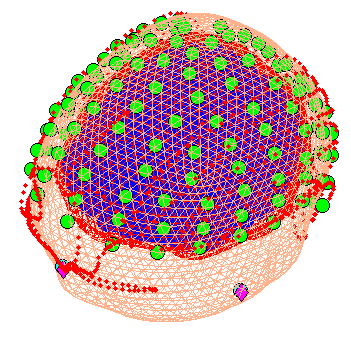
\includegraphics[width=70mm]{multimodal/figures/eeg_coreg.png}
\caption{\em  Graphical output of Co-registration of EEG data, showing (upper panel) cortex (blue), inner skull (red) and scalp (black) meshes, electrode locations (green), MRI/Polhemus fiducials (cyan/magneta), and headshape (red dots).\label{multimodal:fig:8}}
\end{center}
\end{figure}

Note that for these data, the coregistration is not optimal, with several EEG electrodes appearing inside the scalp.  This may be inaccurate Polhemus recording of the headshape or inaccurate surface matching for the scalp mesh, or ``slippage'' of headpoints across the top of the scalp (which might be reduced in future by digitising features like the nose and ears, and including them in the scalp mesh). This is not actually a problem for the BEM calculated below, however, because the electrodes are re-projected to the scalp surface (as a precaution).

Press ``Forward Model'', and select ``EEG BEM''. The first time you do this, there will be a lengthy computation and a large file \texttt{smri\_EEG\_BEM.mat} will be saved in the \texttt{sMRI} directory containing the parameters of the boundary element model (BEM). In the Graphics window the BEM meshes will be displayed with the EEG sensors marked with green asterisks as shown (after rotating to a ``Y-Z'' view using \matlab\ rotate tool) in Figure~\ref{multimodal:fig:2}. This display is the final quality control before the model is used for lead field computation.

\begin{figure}
\begin{center}
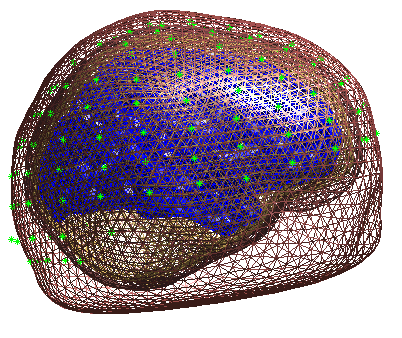
\includegraphics[width=70mm]{multimodal/figures/eeg_forward.png}
\caption{\em BEM meshes with the EEG sensors marked as asterisks.\label{multimodal:fig:2}}
\end{center}
\end{figure}

Press ``Invert'', select ``Imaging'' (i.e, a distributed solution rather than DCM; Kiebel et al (2006)), select ``yes'' to include all conditions (i.e, both the differential and common effects of faces and scrambled faces) and then ``Standard'' to use the default settings.

By default the MSP method will be used. MSP stands for ``Multiple Sparse Priors'' (Friston et al. 2008a), and has been shown to be superior to standard minimum norm (the alternative IID option) or a maximal smoothness solution (like LORETA; the COH option) - see Henson et al (2009a). Note that by default, MSP uses a ``Greedy Search'' (GS) (Friston et al, 2008b), though the standard ReML (as used in Henson et al, 2007) can also be selected via the batch tool (this uses Automatic Relevance Determination - ARD).

The ``Standard'' option uses default values for the MSP approach (to customise some of these parameters, press ``Custom'' instead).

At the first stage of the inversion lead fields will be computed for all the mesh vertices and saved in the file \texttt{SPMgainmatrix\_wmaceMdspm8\_faces\_run1\_1.mat}. Then the actual MSP algorithm will run and the summary of the solution will be displayed in the Graphics window.

Press ``save'' to save the results. You can now explore the results via the 3D reconstruction window. If you type 180 into the box in the bottom right (corresponding to the time in ms) and press ``mip'', you should see an output similar to Figure~\ref{multimodal:fig:9}. This fit explains approx 96\% of the data.

Note the hot-spots in bilateral posterior occipitotemporal cortex, bilateral mid-fusiform, and right lateral ventral temporal. The timecourses come from the peak voxel. The red curve shows the condition currently being shown (corresponding to the ``Condition 1'' toggle bar in the reconstruction window); the grey line(s) will show all other conditions. ``Condition 1'' is the differential evoked responses for faces vs scrambled; if you press the ``condition 1'' toggle, it will change to ``Condition 2'' (average evoked response for faces and scrambled faces), type ``100''ms for the P100, then press ``mip'' again and the display will update (note the colours of the lines have now reversed from before, with red now corresponding to average ERP). 


If you toggle back to ``Condition 1'' and press ``movie'', you will see changes in the source strengths for the differential response over peristimulus time (from the limits 0 to 300ms currently chosen by default).
If you press ``render'' you can get a very neat graphical interface to explore the data (the buttons are fairly self-explanatory). 

You can also explore other inversion options, such as COH and IID (available for the ``custom'' inversion), which you will notice give more superficial solutions (a known problem with standard minimum norm approaches). To do this quickly (without repeating the MRI segmentation, coregistration and forward modelling), press the ``new'' button in the reconstruction window, which by default will copy these parts from the previous reconstruction.

In this final section we will concentrate on how to prepare source data for subsequent statistical analysis (eg with data from a group of subjects).

\begin{figure}
\begin{center}
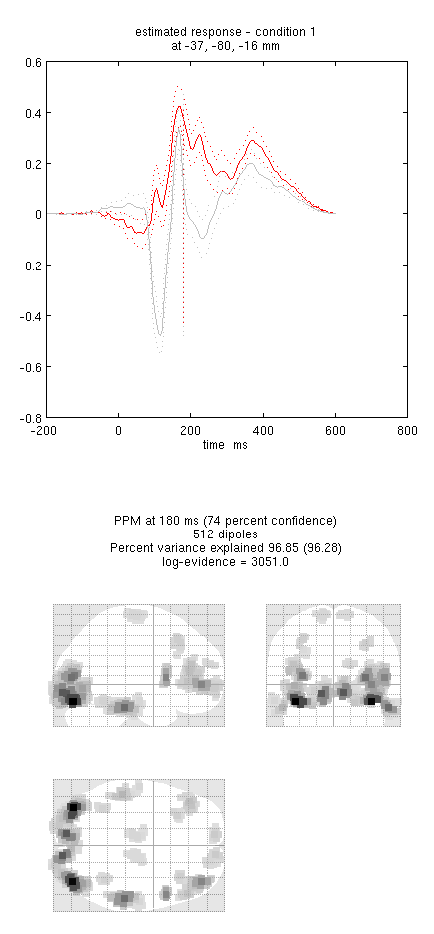
\includegraphics[width=90mm]{multimodal/figures/eeg_msp.png}
\caption{\em Graphical output of an MSP estimation of the differential ERP between faces and scrambled faces at 180ms. \label{multimodal:fig:9}}
\end{center}
\end{figure}

Press the ``Window'' button in the reconstruction window, enter ``150 200'' as the timewindow of interest and keep ``0'' as the frequency band of interest (0 means all frequencies). The Graphics window will then show the mean activity for this time/frequency contrast (top plot) and the contrast itself (bottom plot; note additional use of a Hanning window).

Then press ``Image'' and SPM will write 3D NIfTI images corresponding to the above contrast for each condition:
\begin{verbatim}
    wmaceMdspm8_faces_run1_1_t150_200_f_1.nii
    wmaceMdspm8_faces_run1_1_t150_200_f_2.nii
\end{verbatim}
The last number in the file name refers to the condition number; the number following the dataset name refers to the reconstruction number (i.e. the number in red in the reconstruction window, i.e, \texttt{D.val}, here 1). The reconstruction number will increase if you create a new inversion by pressing ``new''.

The smoothed results for Condition 1 (i.e, the differential evoked response for faces vs scrambled faces) will also be displayed in the Graphics window, see Figure~\ref{multimodal:fig:eegrecon} (after moving the cursor to the right posterior hotspot), together with the normalised structural. Note that the solution image is in MNI (normalised) space, because the use of a canonical mesh provides us with a mapping between the cortex mesh in native space and the corresponding MNI space.

You can also of course view the image with the normal SPM ``Display:image'' option (just the functional image with no structural will be shown), and locate the coordinates of the ``hotspots'' in MNI space. Note that these images contain RMS (unsigned) source estimates (see Henson et al, 2007).
Given that one has data from multiple subjects, one can create a NIFTI file for each. Group statistical analysis can the be implemented with eg. second level t-tests as described earlier in the chapter.


\begin{figure}[h!t]
\begin{center}
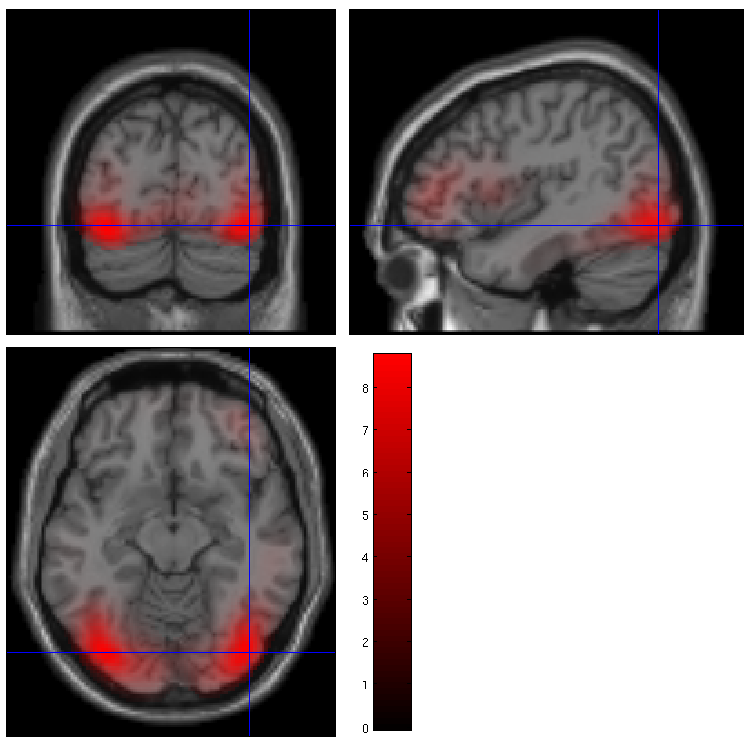
\includegraphics[width=90mm]{multimodal/figures/eeg_recon.png}
\caption{\em 3D reconstruction saved as a smoothed NIfTI image of the differential evoked response for faces vs scrambled faces around the N170. \label{multimodal:fig:eegrecon}}
\end{center}
\end{figure}
